\documentclass{beamer}

\usepackage{cmap}
\usepackage[english,russian]{babel} % add eng,rus(base) package
\usepackage[T1,T2A]{fontenc}        % add eng,rus encoding support
\usepackage[utf8]{inputenc}         % add UTF8 support

% Use it for English document
%\usepackage[utf8]{inputenc} % add UTF8 support
%\usepackage{fontspec}       % to use any font known to the operating system
%\setmainfont{PT Serif}      % set defolt font

\usepackage{amsmath, amsfonts, amssymb, amsthm, mathtools} % add math support

\linespread{1}               % length between str
\setlength{\parindent}{16pt} % red str
\setlength{\parskip}{6pt}   % length between paragraphs

\usepackage[backend=biber, style=authoryear-icomp]{biblatex}
\addbibresource{$HOME/latex-templates/biblio.bib}            % path to bibliography base

\usetheme{Madrid}
\setbeamertemplate{frametitle}[default][center]

\renewcommand{\thefootnote}{\arabic{footnote}}
 % here is document's settings for russian
%\input{$HOME/studyproject/universe/history/preamble-beamer-eng.tex} % here is document's settings for english


\title{Первая Государственная Дума}
\author{Немков Н.М.}
\institute[МГТУ]{МГТУ им. Н.Э. Баумана}
\date{29.02.2024}
\logo{
\includegraphics[width=1cm]{images/logo}}

\begin{document}

\begin{frame}
\maketitle
\end{frame}

\begin{frame}{Содержание}
\tableofcontents
\end{frame}


\begin{frame}

	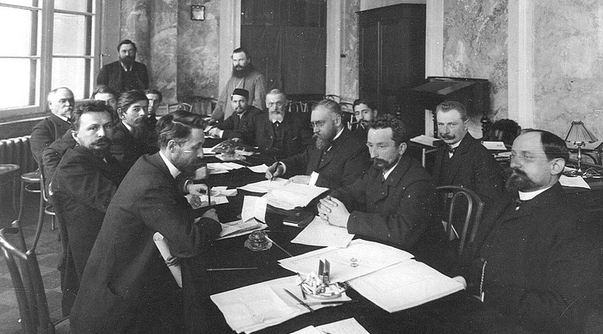
\includegraphics[width=0.9\textwidth]{images/duma-1.png}

	Группа депутатов во время совещания
\end{frame}

\section{Выборы в первую думу}

\begin{frame}{Выборы в первую думу}
	\Large{Женищины, мужчины до 25 лет, военнослужащие и некоторые национальности не имели права голосовать. Также голосование было не равным
	}
\end{frame}

\section{Партии}
\begin{frame}{Партии}
    Выборы в Первую Думу проходили согласно закону от декабря 1905 года. Были учреждены шесть курий:
	\begin{itemize}

		\item землевладельческая --- 1 выборщик на 2 тыс избирателей

		\item городская --- 1 выборщик на 4 тыс избирателей

		\item крестьянская --- 1 выборщик на 30 тыс избирателей

		\item рабочая --- 1 выборщик на 90 тыс избирателей

	\end{itemize}
\end{frame}

\begin{frame}
Распределение депутатов Государственной думы по партиям
	\begin{itemize}

		\item РСДРП --- 10

		\item Трудовики --- 107

		\item Кадеты --- 161

		\item Автономисты --- 70

		\item Октябристы --- 13

		\item Безпартийные --- 100
	\end{itemize}


\end{frame}

\section{}
\begin{frame}{}

	\Large{Главным в работе Государственной Думы был земельный вопрос

	Всего же за время работы депутатов был одобрен один законопроект

	В итоге первая Дума была распущена Николаем II}

\end{frame}

\section{Источники}

\begin{frame}[t]{Источники}
	\large{
	\url{http://duma.gov.ru/duma/about/history/information/}

	\url{https://laservirta.ru/izbiratelnyj-zakon-1907/}

	\url{https://istoriarusi.ru/imper/pervaya-gosudarstbennaya-duma-1906.html}}
\end{frame}


\section{Благоданость}
\begin{frame}
	\centering
	\huge
	Спасибо за внимание!
\end{frame}

\end{document}
